\documentclass[11pt, twoside]{book}
\usepackage[full]{leadsheets}
\usepackage[a4paper,  hmargin=1.5cm, vmargin=3cm, head=14pt, foot=50pt]{geometry}
\usepackage{multicol}
\usepackage[polish]{babel}
\usepackage{array}
\usepackage{graphicx}
\usepackage{hyperref}
\usepackage{tocloft}
%\usepackage[toc]{multitoc}
\usepackage{fancyhdr}
\usepackage{tikzpagenodes}
\usepackage{titlesec}
\usepackage{tabularx}
\usepackage{adjustbox}
\usepackage{tipa}
\usepackage{ifxetex}
\usepackage{changepage}
\usepackage[version=4]{mhchem}
\usepackage[%
    left = „,%
    right = “,%
    leftsub = «,%
    rightsub = »%
]{dirtytalk}

\thispagestyle{empty}

\ifxetex%
    \usepackage{substitutefont}
    \substitutefont{T3}{\rmdefault}{cmr}
\fi

%\usepackage[T1]{fontenc}

\selectlanguage{polish}
\DeclareTranslation{Polish}{leadsheets/chorus}{Ref.}
\DeclareTranslation{Polish}{leadsheets/interlude}{Przej.}
\DeclareTranslation{Polish}{leadsheets/bridge}{Bridge}
\DeclareTranslation{Polish}{leadsheets/lyrics}{tekst}
\DeclareTranslation{Polish}{leadsheets/verse}{Zwr.}
\DeclareTranslation{Polish}{leadsheets/capo}{Capo}
\DeclareTranslation{Polish}{leadsheets/fret}{próg}

% Tytuł spisu treści
\addto\captionspolish{\renewcommand*\contentsname{Jakieś piosenki}}

% Flaga oznaczająca, czy dany utwór ma mieć symbol odnoszący do aneksu
\definesongproperty{annex}

\definesongtitletemplate{custom}{%
    \let\clearpage\relax
    \ifsongmeasuring%
        {\section*}
        {\section}%
        {\songproperty{title}}%
    \begingroup\footnotesize
        \begin{tabular}{%
                @{}
                >{\raggedright\arraybackslash}p{.5\linewidth}
                @{}
                >{\raggedleft\arraybackslash}p{.5\linewidth}
                @{}
            }
            \ifsongproperty{music}{%
                Muzyka: \songproperty{music}
                }{}%
            \ifsongproperty{annex}{%
                &
                \smash{\includegraphics[height=40pt]{images/aneks-ref.png}}
                }{}%
            \ifsongproperty{music}{\\}{\ifsongproperty{annex}{\\}{}}%
            \ifsongproperty{lyrics}{%
                Tekst: \songproperty{lyrics} \\%
                }{}%
            \ifsongproperty{interpret}{%
                Interpretacja: \songproperty{interpret} \\%
                }{}%
            \ifsongproperty{capo}{%
                \capo{} \\%
                }{}%
        \end{tabular}%
        \par
    \endgroup
}

\setleadsheets{%
    title-template = custom,
    verse/numbered,
    remember-chords = false,
    align-chords = {l},
    capo-nr-format = arabic,
    bar-shortcuts
}
\setchords{%
    minor = {lowercase},
    input-notation = german,
    output-notation = german
}

\renewcommand{\chaptermark}[1]{\markboth{#1}{}}

\fancypagestyle{plain}{%
    \fancyhf{}
    \fancyhead[L]{Jakieś piosenki}
    \fancyfoot[LE,RO]{\Large\thepage}
}
\fancypagestyle{szanty}{%
    \pagestyle{plain}
    \fancyhead[R]{Szanty}
    \fancyfoot[LO]{\includegraphics[height=45pt]{images/kolo.png}}
    \fancyfoot[RE]{\includegraphics[height=45pt]{images/kotwica.png}}
}
\fancypagestyle{poezja}{%
    \pagestyle{plain}
    \fancyhead[R]{Poezja śpiewana}
    \fancyfoot[LO]{\includegraphics[height=45pt]{images/wilk.png}}
    \fancyfoot[RE]{\includegraphics[height=45pt]{images/drzewa.png}}
}
\fancypagestyle{pop}{%
    \pagestyle{plain}
    \fancyhead[R]{Pop}
    \fancyfoot[LO]{\includegraphics[height=45pt]{images/gwiazdy.png}}
    \fancyfoot[RE]{\includegraphics[height=45pt]{images/gitara.png}}
}
\fancypagestyle{autorskie}{%
    \pagestyle{plain}
    \fancyhead[R]{Autorskie}
    \fancyfoot[LO]{
\includegraphics[height=45pt]{images/kalamarz.jpeg}}
    \fancyfoot[RE]{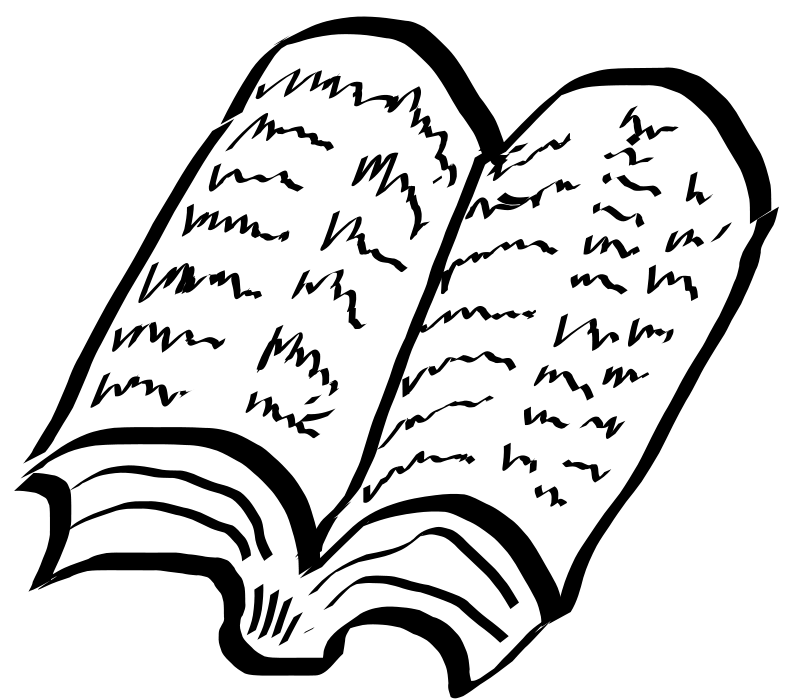
\includegraphics[height=45pt]{images/ksiazka_bazgroly.png}}
}
\fancypagestyle{legendy}{%
    \pagestyle{plain}
    \fancyhead[R]{Legendy, opowieści, ciekawostki}
    \fancyfoot[LO]{\includegraphics[height=45pt]{images/swieczka.png}}
    \fancyfoot[RE]{\includegraphics[height=45pt]{images/fajka.png}}
}

\renewcommand{\cftdot}{\ensuremath{\sim}}
\renewcommand{\cftsecleader}{\cftdotfill{\cftdotsep}}

% Usunięcie numeru rozdziału sprzed numeru sekcji
%\renewcommand{\thesection}{\arabic{section}}

\titleformat{\chapter}[block]{\centering\vspace{6cm}}{}{0pt}{\Huge\bfseries}

\newversetype{riff}[name={Riff}, numbered=false, named=true]

\counterwithin*{footnote}{section}

% Pionowy apostrof do angielskiego i francuskiego
\newcommand{\tqs}{\textquotesingle}

\begin{document}

\begin{titlepage}
    \begin{center}
        \vspace*{5cm}
        
        \includegraphics[height=8cm]{images/front-obrazek.png}

        \vspace{1.5cm}

        \Huge\textbf{Jakieś piosenki}
        
        \vspace{0.5cm}
        
        \large Wydanie pierwsze
        
        \vfill

        \large
        Wydawnictwo Kis Inkris \\
        Warszawa, 2022

        \vspace{0.8cm}

        \footnotesize
        \textit{%
        Gdzie słyszysz śpiew, tam wejdź, tam dobre serce mają \\
        Żli ludzie, wierzaj mi, ci nigdy nie śpiewają} \medskip \\
        Johann Gottfried Seume, \textit{Die Gesänge}

    \end{center}
\end{titlepage}

\pagestyle{plain}

\tableofcontents
\vfill
\renewcommand{\tabularxcolumn}[1]{>{\small}b{#1}}
\begin{adjustbox}{width={\textwidth}, keepaspectratio}
\begin{tabularx}{\textwidth}{%
        @{}
        >{\raggedright\arraybackslash}X
        @{}
        >{\raggedleft\arraybackslash}X
    }
    \footnotesize
    Kamil Dzierżanowski \hfill opracowanie, skład, korekta

    Paweł Kulig \hfill opracowanie
    
    Piotr Wieżel \hfill opracowanie

    \medskip

    Daj śpiewnikowi gwiazdkę na GitHubie:

    \smallskip

    \urlstyle{same}
    \url{https://github.com/dzierzanowski/spiewnik-szant}

    \bigskip

    Dziękujemy za grafiki z Freepik od dgim-studio i pch.vector!

    &

    Pobierz śpiewnik online:

    \smallskip

    \includegraphics[width=3cm]{images/qr.png}
\end{tabularx}
\end{adjustbox}

\chapter{Szanty}
\begin{center}
    \includegraphics[width=0.5\textwidth]{images/wezel.png}
\end{center}
\pagestyle{szanty}
\input{songs/trzy_majtki-24_lutego}
\input{songs/mechanicy_shanty-bitwa}
\input{songs/mietek_folk-chlopcy_z_botany_bay}
\input{songs/trzy_majtki-cztery_piwka}
\input{songs/krzysztof_klenczon-dziesiec_w_skali_beauforta}
\input{songs/ryczace_dwudziestki-few_days}
\input{songs/trzy_majtki-gdzie_ta_keja}
\input{songs/ryczace_dwudziestki-hiszpanskie_dziewczyny}\newpage\pagestyle{szanty}
\input{songs/ryczace_dwudziestki-jasnowlosa}
\input{songs/ekt_gdynia-ja_stawiam}
\input{songs/north_cape-kapitan_kidd}
\input{songs/perly_i_lotry-la_valette}
\input{songs/ekt_gdynia-male_piwo}
\input{songs/mechanicy_shanty-marco_polo}
\input{songs/ekt_gdynia-morze_moje_morze}
\input{songs/artur_andrus-nazywali_go_marynarz}
\input{songs/mechanicy_shanty-pacyfik}
\input{songs/ekt_gdynia-piesn_wielorybnikow}\newpage\pagestyle{szanty}
\input{songs/poszedlem_na_dziob-pij_za_starego}
\input{songs/cztery_refy-pozegnanie_liverpoolu}
\input{songs/cztery_refy-press_gang(branka)}
\input{songs/roman_roczen-przechyly}
\input{songs/zejman_garkumpel-samantha}
\input{songs/hugues_aufray-santiano}
\input{songs/mechanicy_shanty-stara_maui}
\input{songs/ekt_gdynia-stary_bryg}
\input{songs/mechanicy_shanty-stary_wrak}
\input{songs/marek_szurawski-szesnascie_ton}\newpage\pagestyle{szanty}
\input{songs/smugglers-szkuner_im_alone}
\input{songs/the_longest_johns-wellerman}\newpage\pagestyle{szanty}

\chapter{Poezja śpiewana}
\begin{center}
    \includegraphics[width=0.5\textwidth]{images/chatka.jpg}
\end{center}
\pagestyle{poezja}
\input{songs/jacek_kaczmarski-1788}\newpage\pagestyle{poezja}
\input{songs/ekt_gdynia-ballada_na_zle_drogi}
\input{songs/marek_grechuta-dni_ktorych_nie_znamy}\newpage\pagestyle{poezja}
\input{songs/sdm-jak}
\input{songs/tomasz_lewandowski-jaka_jestes}
\input{songs/sdm-jest_juz_za_pozno}
\input{songs/wolna_grupa_bukowina-majster_bieda}
\input{songs/agnieszka_osiecka-nim_wstanie_dzien}
\input{songs/wolna_grupa_bukowina-pejzaze_harasymowiczowskie}
\input{songs/dom_o_zielonych_progach-pojde_w_poloniny}
\input{songs/wolna_grupa_bukowina-sielanka_o_domu}
\input{songs/marek_grechuta-swiecie_nasz}\newpage\pagestyle{poezja}
\input{songs/marcin_przybylowicz-wilcza_zamiec}

\chapter{Pop}
\begin{center}
    \includegraphics[width=0.4\textwidth]{images/pop.png}
\end{center}
\pagestyle{pop}
\input{songs/andrzej_zaucha-bylas_serca_biciem}
\input{songs/brodka-granda}
\input{songs/lao_che-hydropieklowstapienie}
\input{songs/linkin_park-in_the_end}
\input{songs/ed_sheeran-i_see_fire}\newpage\pagestyle{pop}
\input{songs/kobranocka-kocham_cie_jak_irlandie}
\input{songs/edyta_gorniak-kolorowy_wiatr}
\input{songs/dawid_podsiadlo-malociasteczkowy}
\input{songs/monika_brodka-mial_byc_slub}
\input{songs/krzysztof_zalewski-milosc_milosc}
\input{songs/skubas-nie_mam_dla_ciebie_milosci}
\input{songs/jakub_szydlowski-pepe_pan_dziobak}\newpage\pagestyle{pop}
\input{songs/strachy_na_lachy-pila_tango}
\input{songs/romek_buga-piosenka_o_hucie}\newpage\pagestyle{pop}
\input{songs/coma-piosenka_pisana_noca}
\input{songs/breakout-pomaluj_moje_sny}
\input{songs/gotye-premium_boy(somebody)}
\input{songs/vance_joy-riptide}
\input{songs/myslovitz-scenariusz_dla_moich_sasiadow}
\input{songs/czeslaw_niemen-sen_o_warszawie}
\input{songs/david_bowie-space_oddity}
\input{songs/the_kinks-sunny_afternoon}
\input{songs/raz_dwa_trzy-trudno_nie_wierzyc_w_nic}
\input{songs/t_love-warszawa}
\input{songs/happysad-zanim_pojde}

\chapter{Autorskie}
\begin{center}
    
\includegraphics[width=0.4\textwidth]{images/writing_hand.jpeg}
\end{center}
\pagestyle{autorskie}
\newpage
\begin{song}{title={Dzień Wojownika}, music={Ślad}}
    \normalsize
    \begin{multicols}{2}
    \begin{intro}
        \writechord{h7} \writechord{A6} \writechord{GΔ7} \writechord{f#7}
    \end{intro}
    \begin{verse}

	Po^{h7}wiedz mi,^{A6} jak wygląda dz^{GΔ7}ień ^{f#7} \\
	Dzień Wojown^{h7}ika? \\
	Twoja tw^{A6}arz tyle mówi m^{GΔ7}i, \\
	^{f#7}a ja nie umiem z niej cz^{h7}ytać ^{A6} \\
	I ten bl^{GΔ7}ask,^{f#7} blask w twoich ocz^{h7}ach, \\
	jak nagła z nieba r^{A6}osa \\
	Sk^{GΔ7}ąd bierzesz tyle s^{f#7}ił? \medskip

    \end{verse}
    \begin{chorus}
	Jak m^{h7}ożesz twierdzić, ż^{A6}e \\
	m^{GΔ7}oc w słabości d^{f#7}oskonali się? \\
	I wygr^{h7}ywać^{A6}, bo pomaga c^{GΔ7}i \\ 
	Kt^{f#7}oś, kogo nawet nie w^{h7}idać ^{f#7} ^{GΔ7} ^{A6} \medskip
    \end{chorus}
    \begin{verse}
	Po^{h7}wiedz mi,^{A6} jak się widzi św^{GΔ7}iat ^{f#7} \\
	Świat, gdy się w^{h7}ierzy? \\
	Taki św^{A6}iat jest tak obcy m^{GΔ7}i, \\
	^{f#7}a ty nie tracisz nadz^{h7}iei ^{A6} \\
	I ta m^{GΔ7}oc^{A6}, moc w twoim wn^{h7}ętrzu \\
	Nie gubisz nigdy s^{A6}ensu \\
	Sk^{GΔ7}ąd bierzesz t^{f#7}yle sił? \medskip
    \end{verse}
    \begin{chorus}
	Jak m^{h7}ożesz twierdzić, ż^{A6}e \\
	m^{GΔ7}oc w słabości d^{f#7}oskonali się? \\
	I wygr^{h7}ywać, ^{A6} bo pomaga c^{GΔ7}i \\ 
	Kt^{f#7}oś, kogo nawet nie w^{h7}idać ^{f#7} ^{GΔ7} ^{A6} $\times 2$
    \end{chorus}
    \end{multicols}
\end{song}



\newpage
\begin{song}{title={Niezapominajka}, music={Ślad}}
    \normalsize
    \begin{intro}
	\writechord{e} (dwa takty)
    \end{intro}
    \begin{verse}
        M^{e}ija przechodzień witryny sklepowe, mija kwiaciarnie i widzi, że \\
        Tak nienaganne, żywe bez wody, tak niezniszczalne ich życie jest. \medskip
    
        A t^{C}yle jest w n^{D}as z ż^{D}ycia kwiatu \\
        Błęk^{C}itną mam tw^{D}arz i w^{e}ieje wiatr \\
        Nie kł^{C}amię, że m^{D}am w^{D}iele czasu \\
        Pon^{C}iesie mnie t^{D}am, gdzie b^{h7sus}ędzie chciał \medskip
    \end{verse}
    \begin{chorus}
        T^{C}ak, j^{D}ak n^{e}iezapominajka, na tr^{C}aw ziel^{D}onym tl^{e}e \\ 
        Ch^{C}oc^{D}iaż życie to nie bajka, On n^{C}ie zap^{D}omni mn^{e}ie \\
        T^{C}ak, j^{D}ak n^{e}iezapominajka, na tr^{C}aw ziel^{D}onym tl^{e}e \\
        Ch^{C}oc^{D}iaż życie to nie bajka, On n^{C}ie zap^{D}omni mn^{h7sus}ie \medskip
    \end{chorus}
    \begin{verse}
        T^{e}utaj nie mamy witryny i sławy, pewnie uschniemy, gdy zniknie deszcz \\
        Zbyt delikatne są nasze płatki, ale nad nami niebo jest! \medskip

	A t^{C}yle jest w n^{D}as z ż^{D}ycia kwiatu... \\
    \end{verse}
    \begin{chorus}
        T^{C}ak, j^{D}ak n^{e}iezapominajka, na tr^{C}aw ziel^{D}onym tl^{e}e... \\
    \end{chorus}
    \begin{outro}
        A t^{C}yle jest w n^{D}as z ż^{D}ycia kwiatu \\
        Błęk^{C}itną mam tw^{D}arz i w^{e}ieje wiatr \\
        Nie kł^{C}amię, że m^{D}am w^{D}iele czasu \\
        Pon^{C}iesie mnie t^{D}am, gdzie b^{e}ędzie chciał 
    \end{outro}
\end{song}


\chapter{Legendy, opowieści, ciekawostki}
\begin{center}
    \includegraphics[width=0.4\textwidth]{images/bosman.png}
\end{center}
\pagestyle{legendy}
\input{legendy}

% Ostatnia strona parzysta pusta, żeby nie było tekstu na odwrocie
\clearpage{\mbox{}\pagestyle{empty}\cleardoublepage}

\end{document}
